% ~ 12 pages
\chapter{Identification of Hadronically Decaying $\tau$-Leptons (BDT)}
\label{sec:bdt}

TODOs:
\begin{itemize}
\item Working point efficiencies for pt and mu
\item Rejection for full pt range
\item Plot 2nd order effects (e.g. ptRatioEflowApprox vs.\ mEflowApprox (1P) or
  massTrkSys vs.\ EMPOverTrkSysP (3P))
\item Partial dependence plots
\item trFlightPathSig: why the negative sign?
\item Understand the rejection vs.\ pt curve. Why does the rejection drop (is it
  because rejection is enhanced due to pile-up fakes)? Why does rejection
  increase again for high pt?
\item Properly define Rejection = Inverse background efficiency
\item BDT is optimised for a 'gammatautau'-like spectrum (focused on improving
  rejection at low pt)
\end{itemize}

\section{Features of Hadronically Decaying Tau Leptons}
\label{sec:features_tau_decay}

Features of hadronically decaying $\tau$-leptons vs. Quark/Gluon initiated jets:
\begin{itemize}
\item Low multiplicity (QCD jets usually have a lot of tracks)
\item Isolated tracks and narrow showers
\item Measurable decay length with proper lifetime of
  $\tau = \SI{290.3 +- 0.5}{\femto\second}$ \cite{pdg} and following from that
  $c \tau = \SI{87.0 +- 0.2}{\micro\metre}$ with $\beta \gamma = 10$ which
  corresponds to a roughly \SI{18}{\giga\electronvolt} tau the mean decay length
  is of the order of a millimetre and allows secondary vertex reconstruction or
  employing the impact parameter for 1-prong taus (sub-millimetre resolution).
\item Invariant mass bounds for decay products
\end{itemize}


\section{Event Simulation, Reweighting and Preselection}
\label{sec:bdt_eventsim}

\todo[inline]{Signal}
For training and performance evaluation simulated data is used. For tau
performance trainings and tunings a sample created by the process
$\gamma^* \rightarrow \tau \tau \, \text{(hadr.)}$ is used, where at
generator-level leptonic decays of the tau is disabled. Moreover interference
with and on-/ off-shell production of the $\mathrm{Z}^0$ boson is disabled. The
reason for not using a sample employing the Drell--Yan process including
interference and on- / off-shell production of the $\mathrm{Z}^0$ boson is that
the tau polarisation changes for di-tau invariant masses close to the
$\mathrm{Z}$-mass whereas unpolarised taus are desired. Moreover the di-tau mass
spectrum is smooth and decreasing without increased statistics close to the
$\mathrm{Z}$ mass which is not needed for performance studies.

The background for the identification studies is given by dijet samples up to
\SI{1800}{\giga\electronvolt} (JZ1W - JZ6W). \todo[inline]{Finish this; Fraction
  of the mass slices -- high pt enhanced; why not JZ0W -- very low pt / not
  passing 20 GeV cut?}

Baseline tau selection:
\begin{itemize}
\item $p_\text{T} > \SI{20}{\giga\electronvolt}$ (sufficient for most analyses)
\item Exclude calorimeter transition region $1.37 < |\eta| < 1.52$
\item Require tracker acceptance region $|\eta| < 2.5$
\item One or three reconstructed tracks
\item Truth-matching for signal events ($p_\text{T}$, $\eta$ and
  $N_\text{track}$ selection also at truth-level)
\end{itemize}

Size of the pre-production samples after baseline tau selection:
\begin{itemize}
\item Signal: 13.3 M (1P: 10.5 M, 3P: 2.8 M)
\item Background: 22.1 M (1P: 6.6 M, 3P: 15.5 M)
\end{itemize}

\todo[inline]{Interesting plots: pt spectra, mu-distribution}

\todo[inline]{Reweighting}

A full summary of the datasets is given in appendix \todo{Reference}.

\section{Description of the Tau-Identification Procedure}
\label{sec:bdt_tauid}

\subsection{Features (Predictors, Dependent Variables, Input Variables)}
\label{sec:bdt_features}

\begin{figure}[ht]
  \begin{subfigure}[t]{0.48\textwidth}
    \centering
    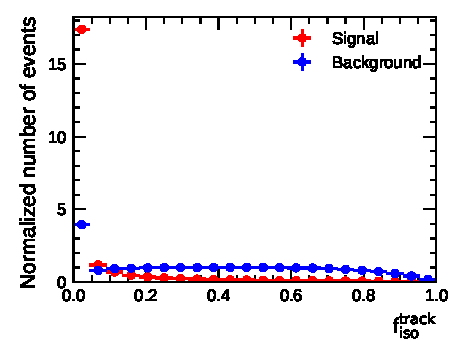
\includegraphics{./figures/baseline_bdt_vars/1p/SumPtTrkFrac.pdf}
    \subcaption{Momentum fraction of isolation tracks (1-prong)}
  \end{subfigure}\hfill
  \begin{subfigure}[t]{0.48\textwidth}
    \centering
    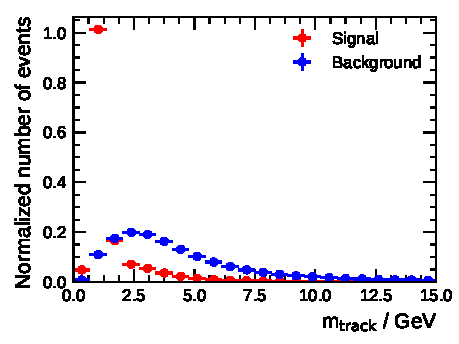
\includegraphics{./figures/baseline_bdt_vars/3p/massTrkSys.pdf}
    \subcaption{Mass of the track system (3-prong)}
  \end{subfigure}
  \caption{}
  \label{fig:bdt_discriminants}
\end{figure}

\begin{table}[ht]
  \centering
  \begin{tabular}{ccc}
  \toprule
  Variable & 1-track & 3-track \\
  \midrule
  \smash{$f _\text{cent}$} & \textbullet & \textbullet \\
  \smash{$f_\text{leadtrack}^{-1}$} & \textbullet & \textbullet \\
  \smash{$R_\text{track}$} & \textbullet & \textbullet\\
  \smash{$\Delta R_\text{max}$} & & \textbullet \\
  \smash{$| S_\text{leadtrack} |$} & \textbullet & \\
  \smash{$S_\text{T}^\text{flight}$} & & \textbullet \\
  \bottomrule
\end{tabular}\hspace*{2em}
\begin{tabular}{ccc}
  \toprule
  Variable & 1-track & 3-track \\
  \midrule
  \smash{$f_\text{iso}^\text{track}$} & \textbullet & \\
  \smash{$f_\text{EM}^\text{track-HAD}$} & \textbullet & \textbullet \\
  \smash{$f_\text{track}^\text{EM}$} & \textbullet & \textbullet \\
  \smash{$p_\text{T}^\text{EM+track} / p_\text{T}$} & \textbullet & \textbullet \\
  \smash{$m_\text{EM+track}$} & \textbullet & \textbullet \\
  \smash{$m_\text{track}$} & & \textbullet \\
  \bottomrule
\end{tabular}

%%% Local Variables:
%%% mode: latex
%%% TeX-master: "../mythesis"
%%% End:

  \caption{Variables used for identification}
  \label{tab:baseline_variables}
\end{table}

\todo{Define what is electromagnetic energy for taus (Presampler, EM1, EM2)}
\todo{Backref to reco chapter: track classification, axes}

Input variables:
\begin{description}
\item[Central energy fraction ($f_\text{cent}$):] Fraction of transverse energy
  (EM scale) deposited in calorimeter cells with a barycentre in a cone of
  radius $\Delta R < 0.1$, and cells in a cone of radius $\Delta R < 0.2$ with
  respect to the reconstructed tau axis \todo{intermediate axis}. The
  calorimeter cells must be matched to a \emph{TopoCluster}.

\item[Inverse momentum fraction of the leading track
  ($f_\text{leadtrack}^{-1}$):] Fraction of transverse energy (EM scale)
  deposited in calorimeter cells (matched to \emph{TopoClusters}) with a
  barycentre in a cone of radius~$\Delta R < 0.2$ with respect to the tau axis
  \todo{intermediate axis} and the transverse momentum of the highest momentum
  track classified as \emph{charged} according to the track classification
  \todo{ref}.

\item[Track radius ($R_\text{track}$):] Mean $\Delta R$-distance of the
  tau axis \todo{intermediate axis} and tracks classified as \emph{charged}
  weighted by the transverse momentum~$p_\text{T}$ of each track.

\item[Maximum track $\Delta R$ ($\Delta R_\text{max}$):] Maximum
  $\Delta R$-distance of all tracks classified as \emph{charged} with respect to
  the tau axis \todo{intermediate axis}. Equivalent to $R_\text{track}$
  for 1-prong hadronic tau decays.

\item[Transverse impact parameter significance of the leading track
  ($| S_\text{leadtrack} |$):] Absolute value of the transverse impact
  parameter~$d_0$ of the leading \emph{charged} track with respect to the
  reconstructed primary vertex divided by its uncertainty estimate from the
  track and vertex fit.

\item[Transverse flight path significance ($S_\text{T}^\text{flight}$):]
  Distance between secondary vertex reconstructed using tracks classified as
  \emph{charged} and primary vertex in the transverse plane divided by the
  estimated uncertainty from the secondary vertex fit.

\item[Momentum fraction of isolation tracks ($f_\text{iso}^\text{track}$):]
  Transverse momentum~$p_\text{T}$ sum of \emph{modified isolation} tracks
  divided by the transverse momentum sum of \emph{modified isolation} and
  \emph{charged} tracks.

\item[EM energy fraction of charged pions ($f_\text{EM}^\text{track-HAD}$):]
  Energy deposited by charged pions in the electromagnetic part of the
  calorimeter estimated by subtracting the energy contained in the hadronic part
  of \emph{TopoClusters} from the energy of the track-system given by the sum of
  track momenta. This energy is divided by the energy contained in the
  electromagnetic part of calorimeter clusters. All cluster energies are
  calibrated at LC scale.

\item[Ratio of EM energy and track momentum ($f_\text{track}^\text{EM}$):]
  Energy deposited as part of \emph{TopoClusters} of the reconstructed jet in
  the electromagnetic part of the calorimeter (Presampler, EM1 \& EM2)
  calibrated at LC scale, divided by the momentum sum of tracks classified as
  \emph{charged}.

\item[Fraction of track-plus-EM-system $p_\text{T}$
  ($p_\text{T}^\text{EM+track} / p_\text{T}$):] Transverse momentum of the
  visible tau decay estimated from the four-momentum sum of \emph{charged}
  tracks (assuming $\pi^\pm$ mass) and up to two of the most-energetic clusters
  (assuming zero mass) in the electromagnetic part of the calorimeter divided by
  the transverse momentum of the reconstructed tau at LC scale.

\item[Mass of the track-plus-EM-system ($m_\text{EM+track}$):] Invariant mass of
  the visible tau decay estimated from the four-momentum sum of \emph{charged}
  tracks (assuming $\pi^\pm$ mass) and up to two of the most-energetic clusters
  (assuming zero mass) in the electromagnetic part of the calorimeter.

\item[Mass of the track system ($m_\text{track}$):] Invariant mass of
  the system consisting of tracks classified as \emph{charged} using a $\pi^\pm$ mass
  hypothesis.
\end{description}


\begin{align*}
  N_\text{trees} &= 100 & d_\text{tree} &= 8 & \beta &= 0.2 \\
  f_\text{node}^\text{min} &= \SI{0.1}{\percent} & N_\text{cuts} &= 200
\end{align*}
as well as \texttt{UseYesNoLeaf} and no pruning.

Transformations? highly skewed and long-tailed distributions

\todo{Show 2D plot of signal \& background e.g. massTrkSys vs. EMPOverTrkSysP to
  motivate the use of MVA methods / BDTs}

\section{Hyperparameter Optimisation}
\label{sec:bdt_hyperparam}

TMVA \cite{tmva}.

Quickly describe previous setup.

Before proceeding to feature selection a reliable hyperparameter setup has to be
found.

Pick the best-performing BDT \& a good compromise between 'overtraining' and
performance.

Optimised for tight efficiency w/o subsampling:
\begin{itemize}
\item \textbf{Best performance 1P:} MaxDepth: 16, MinNodeSize: 0.01, NTrees:
  400, Shrinkage: 0.05, ratio: 0.997 \textrightarrow alg 244
\item \textbf{Compromise 1P:} MaxDepth: 8, MinNodeSize: 0.1, NTrees: 400,
  Shrinkage: 0.1, sumsampling: 50\%, ratio: 0.977 \textrightarrow alg 321
\item \textbf{Best performance 3P:} MaxDepth: 16, MinNodeSize: 0.01, NTrees:
  400, Shrinkage: 0.4, ratio: 0.998 \textrightarrow 259
\item \textbf{Compromise 3P:} MaxDepth: 6, MinNodeSize: 0.1, NTrees: 800,
  Shrinkage: 0.4, ratio: 0.964 \textrightarrow alg 327
\end{itemize}

\subsection{Boosting Algorithm}
\label{sec:bdt_boosting}
AdaBoost \textrightarrow GradBoost

\begin{figure}[ht]
  \begin{subfigure}[t]{0.48\textwidth}
    \centering
    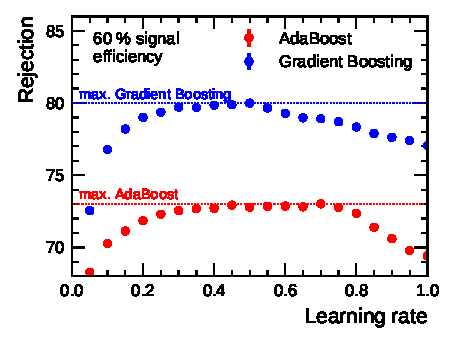
\includegraphics{./figures/bdt_perf/boosting.pdf}
    \subcaption{Impact of the boosting algorithm. $N_\text{trees} = 100$,
      $d_\text{tree} = 8$, $f_\text{node}^\text{min} = \SI{0.1}{\percent}$ and
      varying the learning rate $\beta$~(\emph{AdaBoost}) and $\eta$~(Gradient
      Boosting) respectively.}
    \label{fig:bdt_boosting_alg}
  \end{subfigure}\hfill
  \begin{subfigure}[t]{0.48\textwidth}
    \centering 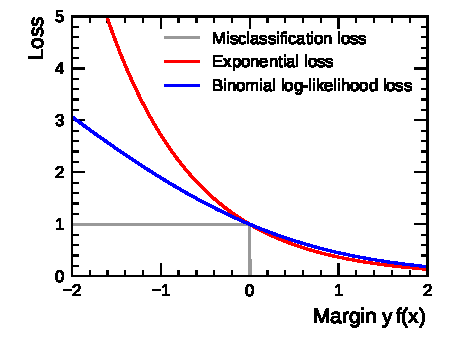
\includegraphics{./figures/theory/boosting_loss.pdf}
    \subcaption{Loss function vs.\ margin adapted from \cite{esl}. Class label
      $y \in \{-1, 1\}$ (signal: 1 / background: -1) and $f(x) \in [-1, 1]$ the
      BDT response.}
    \label{fig:boosting_loss}
  \end{subfigure}
  \caption{Loss function investigation}
\end{figure}

\todo{Why no full optimisation of the hyperparameters?}

\subsection{Exhaustive Grid Search}
\label{sec:bdt_grid_search}

\begin{align*}
  N_\mathrm{trees} &\in \{25, 50, 100, 200, 400, 800\} &
  d_\mathrm{tree} &\in \{4, 6, 8, 12, 16\} \\
  \eta &\in \{0.05, 0.1, 0.2, 0.4\} &
  f_\mathrm{node}^\mathrm{min} &\in \{\SI{0.01}{\percent}, \SI{0.1}{\percent},\SI{1.0}{\percent}\} \\
  f_\text{bag} &\in \{\text{None}, \SI{50}{\percent} \}
\end{align*}
Total of $6 \times 5 \times 4 \times 3 \times 2 = 720$

Explain why for 1-prong a subsampling model is better than for 3-prong. The
1-prong case seems to be limited by background statistics while the 3-prong case
is limited by signal statistics. Could the reason for the preferred subsampling
models in the 1-prong case be the low statistics for the background? Why?

Explain that the 16 depth trees are not of depth 16 in most cases because it is
limited by MinNodeSize. Assuming the data is split in equal parts for each
binary split then the effective depth is roughly
$d = \log_2(\SI{100}{\percent} / \SI{0.1}{\percent}) \approx 10$.

Reasons for using the 'less overtrained' example:
\begin{itemize}
\item More robust to potential decreases in number of training examples for
  future tunings
\item BDT fits statistical fluctuations (why is this bad when we see an overall
  improvement in performance? how does this fit in with the NN studies where
  this is often the case?)
\item Tuning of downstream algorithms on same sample (algorithms learn overly
  optimistic Tau-ID)
\end{itemize}

TMVA Grid Search
XGBoost (?)
Comparison with previous setup

\begin{figure}[ht]
  \begin{subfigure}[t]{0.48\textwidth}
    \centering
    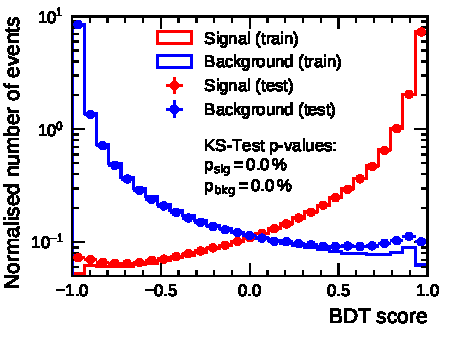
\includegraphics{./figures/bdt_perf/scores/grid_1p0304.pdf}
    \subcaption{Overtrained example (BDT A):
      \mbox{$N_\text{Trees} = 800$},
      \mbox{$d_\text{Tree} = 16$},
      \mbox{$\nu = 0.05$, $f_\text{min.}^\text{Node} = \SI{0.01}{\percent}$},
      no bagging
    }
  \end{subfigure}\hfill
  \begin{subfigure}[t]{0.48\textwidth}
    \centering
    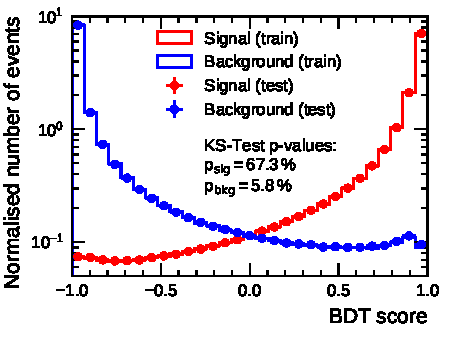
\includegraphics{./figures/bdt_perf/scores/grid_1p_subsampling0269.pdf}
    \subcaption{Good training (BDT B):
      \mbox{$N_\text{Trees} = 400$},
      \mbox{$d_\text{Tree} = 8$},
      \mbox{$\nu = 0.1$, $f_\text{min}^\text{Node} = \SI{0.1}{\percent}$},
      \mbox{$f_\text{bag} = \SI{50}{\percent}$}
    }
  \end{subfigure}
  \caption{'Overtraining' visible on the edges of the BDT score distribution
    (1-prong)}
  \label{fig:bdt_1p_scores}
\end{figure}

\begin{figure}[ht]
  \begin{subfigure}[t]{0.48\textwidth}
    \centering
    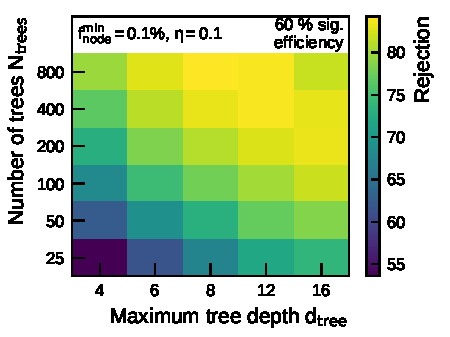
\includegraphics{./figures/bdt_perf/gridsearch_1p/scan_MaxDepth_NTrees.pdf}
    \subcaption{Bla}
  \end{subfigure}\hfill
  \begin{subfigure}[t]{0.48\textwidth}
    \centering
    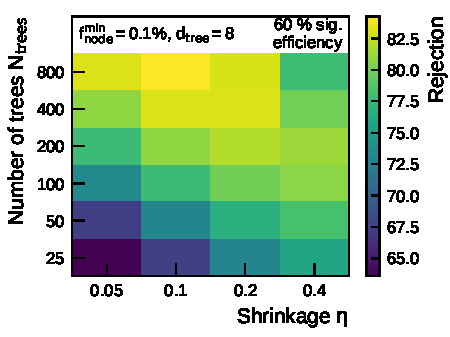
\includegraphics{./figures/bdt_perf/gridsearch_1p/scan_Shrinkage_NTrees.pdf}
    \subcaption{Blabla}
  \end{subfigure}
  \begin{subfigure}[t]{0.48\textwidth}
    \centering
    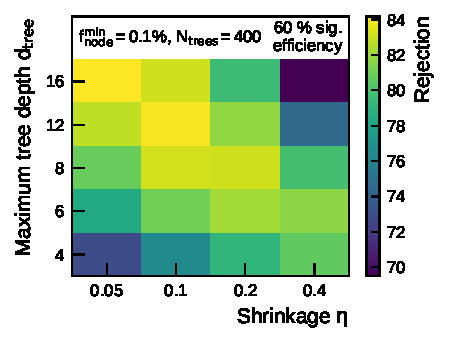
\includegraphics{./figures/bdt_perf/gridsearch_1p/scan_Shrinkage_MaxDepth.pdf}
    \subcaption{Blablabla}
  \end{subfigure}\hfill
  \begin{subfigure}[t]{0.48\textwidth}
    \centering
    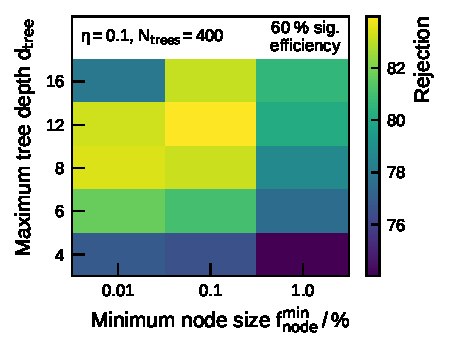
\includegraphics{./figures/bdt_perf/gridsearch_1p/scan_MinNodeSize_MaxDepth.pdf}
    \subcaption{Blablablabla}
  \end{subfigure}
  \caption{Rejection as a function of the hyperparameters. Uses
    \SI{50}{\percent} subsampling. (1-prong). \mytodo{KS-Probability as
      comparison}}
  \label{fig:hyperparameter_scan_1p}
\end{figure}

\begin{figure}[ht]
  \begin{subfigure}[t]{0.48\textwidth}
    \centering
    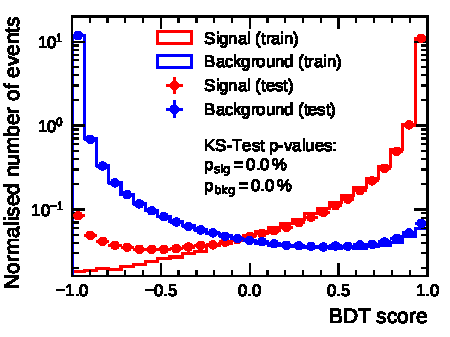
\includegraphics{./figures/bdt_perf/scores/grid_3p0317.pdf}
    \subcaption{Overtrained example (BDT A):
      \mbox{$N_\text{Trees} = 800$},
      \mbox{$d_\text{Tree} = 16$},
      \mbox{$\nu = 0.1$, $f_\text{min.}^\text{Node} = \SI{0.01}{\percent}$},
      no bagging
    }
  \end{subfigure}\hfill
  \begin{subfigure}[t]{0.48\textwidth}
    \centering
    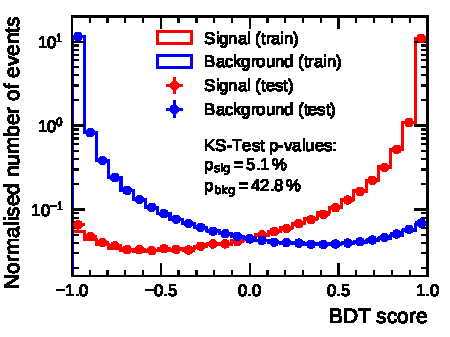
\includegraphics{./figures/bdt_perf/scores/grid_3p0327.pdf}
    \subcaption{Good training (BDT B):
      \mbox{$N_\text{Trees} = 800$},
      \mbox{$d_\text{Tree} = 6$},
      \mbox{$\nu = 0.4$, $f_\text{min}^\text{Node} = \SI{0.1}{\percent}$},
      \mbox{$f_\text{bag} = \text{None}$}
    }
  \end{subfigure}
  \caption{'Overtraining' visible on the edges of the BDT score distribution
    (3-prong)}
  \label{fig:bdt_3p_scores}
\end{figure}

\begin{figure}[ht]
  \begin{subfigure}[t]{0.48\textwidth}
    \centering
    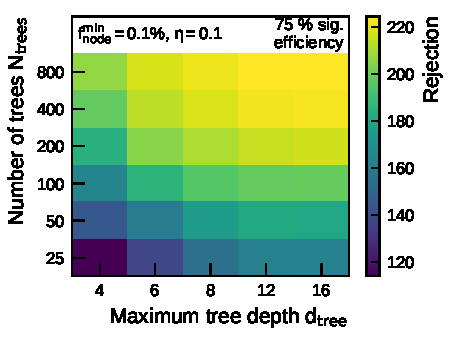
\includegraphics{./figures/bdt_perf/gridsearch_3p/scan_MaxDepth_NTrees.pdf}
    \subcaption{Bla}
  \end{subfigure}\hfill
  \begin{subfigure}[t]{0.48\textwidth}
    \centering
    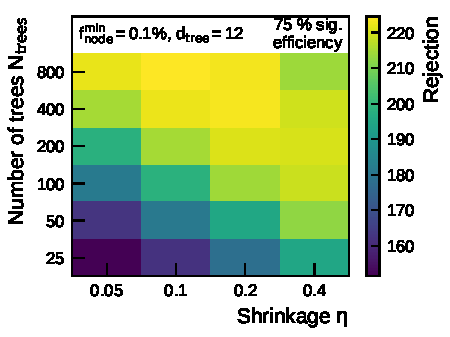
\includegraphics{./figures/bdt_perf/gridsearch_3p/scan_Shrinkage_NTrees.pdf}
    \subcaption{Blabla}
  \end{subfigure}
  \begin{subfigure}[t]{0.48\textwidth}
    \centering
    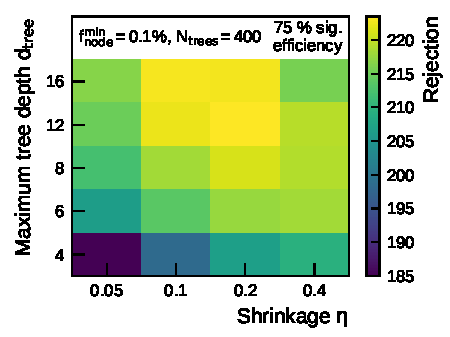
\includegraphics{./figures/bdt_perf/gridsearch_3p/scan_Shrinkage_MaxDepth.pdf}
    \subcaption{Blablabla}
  \end{subfigure}\hfill
  \begin{subfigure}[t]{0.48\textwidth}
    \centering
    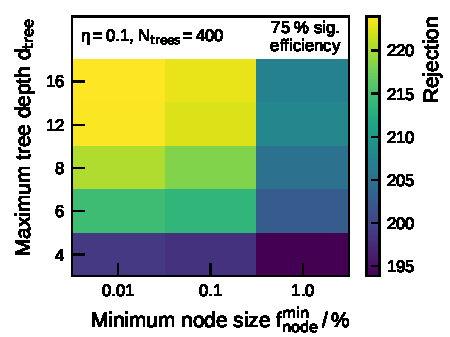
\includegraphics{./figures/bdt_perf/gridsearch_3p/scan_MinNodeSize_MaxDepth.pdf}
    \subcaption{Blablablabla}
  \end{subfigure}
  \caption{Rejection as a function of the hyperparameters. Not using
    subsampling. (3-prong). \mytodo{Not as prone to overfitting? Why? This shows
      the performance on the background sample (does it though? its rejection at
      45\% efficiency) which is less overtrained than the signal sample due to
      higher 3-prong stats for background.} \mytodo{Move bottom two plots to
      appendix.}}
  \label{fig:hyperparameter_scan_3p}
\end{figure}

Description of what is seen in the scan:
\begin{itemize}
\item Strong dependence of $N_\text{trees}$ and $d_\text{tree}$: low number
  shallow trees leads to underfitting; high number of deep trees starts to
  degrade performance due to overfitting
\item Strong dependence of shrinkage and number of trees: Very narrow maximum in
  feature space - shrinkage has to be tuned for the number of trees. Significant
  overfitting in high shrinkage high ntree region.
\item Maximum tree depth vs shrinkage: Deep trees need low shrinkage to avoid
  overfitting and vice versa for underfitting.
\item Maximum tree depth vs minnodesize: Critical parameter to set correctly. If
  set too large severe underfitting is observed. For small minimum node sizes
  one has to be careful to not set the tree depth too high since minimum node
  size is the depth limiter in most cases. One tuning strategy could be to set
  the tree depth to very large values and just limit using minimum node size but
  this would require fine tuning for different sample sizes.
\end{itemize}

\begin{figure}[ht]
  \begin{subfigure}[t]{0.48\textwidth}
    \centering
    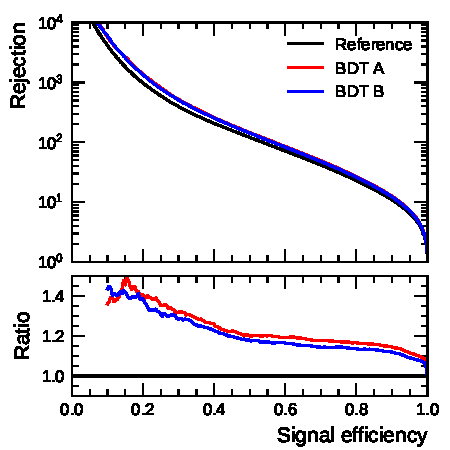
\includegraphics{./figures/bdt_perf/roc/bdt_1p_comparison.pdf}
    \subcaption{1-prong}
    \label{fig:bdt_1p_roc}
  \end{subfigure}\hfill
  \begin{subfigure}[t]{0.48\textwidth}
    \centering
    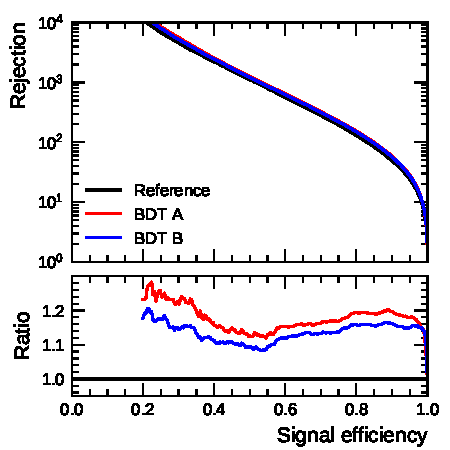
\includegraphics{./figures/bdt_perf/roc/bdt_3p_comparison.pdf}
    \subcaption{3-prong}
    \label{fig:bdt_3p_roc}
  \end{subfigure}
  \caption{\emph{ROC}-Curves. \mytodo{Rule of thumb? For 10 percent signal
      efficiency which factor of rejection do we get?}}
\end{figure}

The one-prong BDT is optimised for efficiency of the tight working-point (in the
scan no flattening was applied). However the 3-prong BDT was optimised for the
loose working-point, because the rejection of the 3-prong ID is roughly one
order of magnitude larger thus the tight working-point is not a stable metric
considering the size of the available background sample.

In partial dependence plots you can see the nonlinear decision boundaries.

\subsection{Working Points}
\label{sec:bdt_working_points}

\begin{figure}[ht]
  \begin{subfigure}[t]{0.48\textwidth}
    \centering
    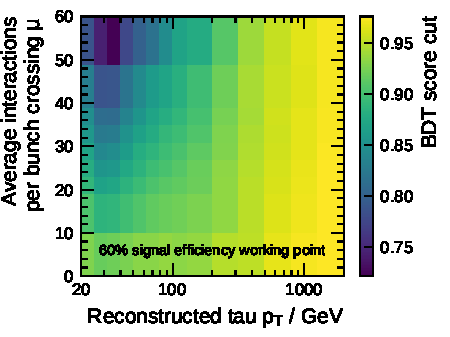
\includegraphics{./figures/bdt_perf/working_points/grid_1p_subsampling0269_wp.pdf}
    \subcaption{1-prong}
  \end{subfigure}\hfill
  \begin{subfigure}[t]{0.48\textwidth}
    \centering
    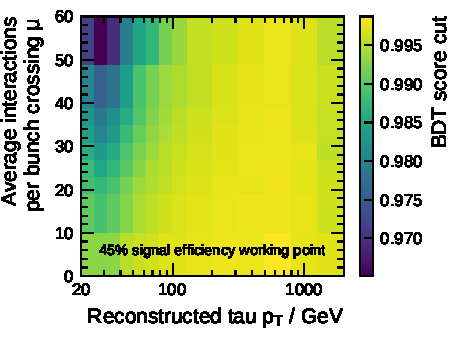
\includegraphics{./figures/bdt_perf/working_points/grid_3p0327_wp.pdf}
    \subcaption{3-prong}
  \end{subfigure}
  \caption{Working points (BDT A)}
\end{figure}

Working points (Gammatautau -- Ztautau)

Signal efficiencies 1P (3P):
\begin{itemize}
\item Very Loose: 95\% (95\%)
\item Loose: 85\% (75\%)
\item Medium: 75\% (60\%)
\item Tight: 60\% (45\%)
\end{itemize}

\begin{figure}[ht]
  \begin{subfigure}[t]{0.48\textwidth}
    \centering
    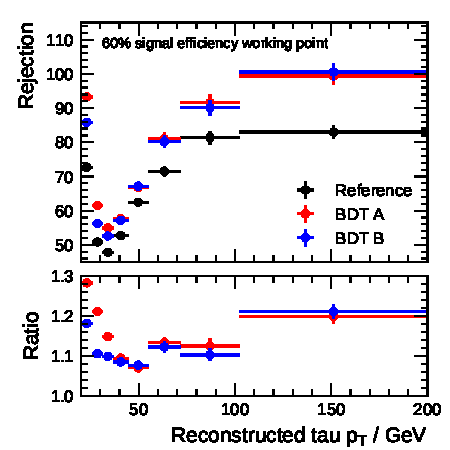
\includegraphics{./figures/bdt_perf/rejection/post_gridsearch_1p/rejection_tight.pdf}
    \subcaption{1-prong (tight)}
  \end{subfigure}\hfill
  \begin{subfigure}[t]{0.48\textwidth}
    \centering
    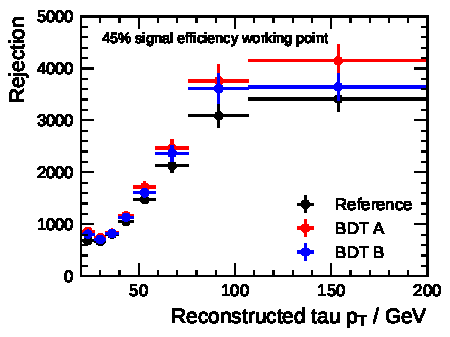
\includegraphics{./figures/bdt_perf/rejection/post_gridsearch_3p/rejection_tight.pdf}
    \subcaption{3-prong (tight)}
  \end{subfigure}
  \caption{Working points (BDT A) \mytodo{Larger pt range in appendix}.
    \mytodo{Ratio is bootstrapped due to highly correlated errors}}
\end{figure}


\begin{itemize}
\item Working point: constant signal efficiency in different pt-regimes and
  pile-up environments. Rejection definitely not flat then!
\item Overall tighter cut for high $p_\text{T}$. Why?
\item Significant degradation at low $p_\text{T}$ for high pile-up. Why?
\item Overall slight improvement for lower pile-up scenarios. Why?
\item Show signal efficiency vs pt and mu
\end{itemize}

\section{Feature Selection}
\label{sec:bdt_feature_selection}

\subsection{Transverse Momentum Dependency of Features}
\label{sec:bdt_incl_pt}

\begin{figure}[ht]
  \begin{subfigure}[t]{0.48\textwidth}
    \centering
    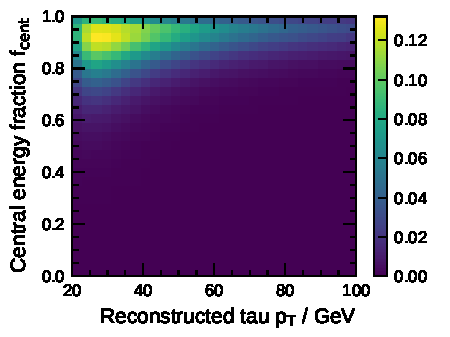
\includegraphics{./figures/bdt_perf/cent_frac_vs_pt_sig.pdf}
    \subcaption{Signal}
  \end{subfigure}\hfill
  \begin{subfigure}[t]{0.48\textwidth}
    \centering
    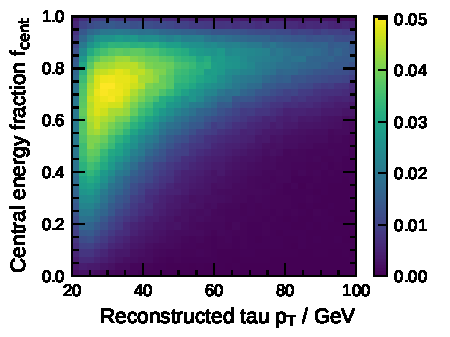
\includegraphics{./figures/bdt_perf/cent_frac_vs_pt_bkg.pdf}
    \subcaption{Background}
  \end{subfigure}
    \caption{$p_\text{T}$-dependency of the central energy fraction.}
  \label{fig:bdt_pt_dependency}
\end{figure}

A lot of the input features have (at least a small) dependency with the
reconstructed $p_\text{T}$ changing the separation of signal and background in
the features as a function of $p_\text{T}$. This effect has a large impact on
the overall isolation of the shower in the calorimeter and the tracks. An
example of this is the central energy fraction $f_\text{cent}$ shown in figure
\ref{fig:bdt_pt_dependency}. While the energy for signal events is mostly
contained in the cone of size $\Delta R < 0.1$ there are significant
contributions to the $0.1 < \Delta R < 0.2$ annulus for dijets reconstructed as
low $p_\text{T}$ tau candidates. To take advantage of the varying separation of
the input features in different $p_\text{T}$-regions the transverse momentum can
be included as an input to the BDT. It is important that the signal and
background samples used for training are reweighted such that no discrimination
purely based on the $p_\text{T}$-spectra of the samples is possible. For the use
of tau-identification in analyses the working point efficiencies in data must be
determined in a tag-and-probe measurement. For reconstructed taus with
transverse momenta greater than \SI{100}{\giga\electronvolt} there is limited
statistics. In practice the measured efficiencies need to be extrapolated to
higher $p_\text{T}$-regions and therefore it should be avoided to have an
explicit $p_\text{T}$-dependence in the BDT above this threshold (an implicit
dependency due to correlations of the regular features like the central energy
fraction can not be avoided). This is realised by \emph{clamping} the transverse
momentum
\begin{align*}
  p_\text{T}^\text{clamp} = \min(p_\text{T}, \SI{100}{\giga\electronvolt})
\end{align*}
and using this as an input to the BDT.

\begin{table}[htb]
  \centering
  \begin{tabular}{
  l
  p{1.5cm}
  S[table-format=1.1(1)]
  S[table-format=1.1(1)]
  S[table-format=1.1(1)]
  }
  \toprule
  & \multirow{2}{*}[-0.15em]{Variable} & \multicolumn{3}{c}{relative rejection gain / \si{\percent}} \\
  \cmidrule{3-5}
  & & {tight} & {medium} & {loose}\\
  \midrule
  \multirow{2}{*}{\vspace*{-0.2em}1-prong} & $p_\text{T}$ & 4.3 +- 0.4 & 4.4 +- 0.3 & 5.6 +- 0.2 \\[0.2em]
  & $p_\text{T}^\text{clamp}$ & 3.5 +- 0.3 & 3.8 +- 0.3 & 4.9 +- 0.2 \\
  \midrule
  \multirow{3}{*}{\vspace*{-0.4em}3-prong} & $p_\text{T}$ & 2.7 +- 0.9 & 3.9 +- 0.6 & 3.1 +- 0.3 \\[0.2em]
  & $p_\text{T}^\text{clamp}$ & 2.3 +- 0.9 & 3.6 +- 0.5 & 3.1 +- 0.3 \\[0.2em]
  & $f_\text{iso}^\text{track}$ & 3.0 +- 1.0 & 5.6 +- 0.6 & 6.6 +- 0.5 \\
  \bottomrule
\end{tabular}

%%% Local Variables:
%%% mode: latex
%%% TeX-master: "../mythesis"
%%% End:

  \caption{New variables}
  \label{tab:bdt_new_variables}
\end{table}

\subsection{Variable Importance}
\label{sec:bdt_var_importance}

\todo[inline]{Recursive Feature Elimination (also TMVA ranking?); Input variable
  correlations;}

\begin{figure}[ht]
  \begin{subfigure}[t]{0.33\textwidth}
    \centering
    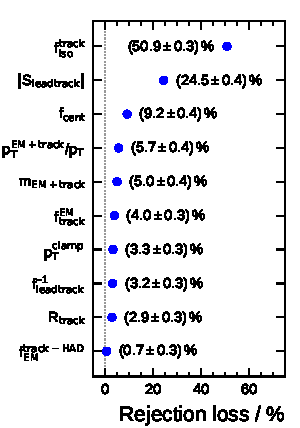
\includegraphics{./figures/bdt_perf/var_importance/1p_iter1.pdf}
    \subcaption{Iteration 1 (1-prong)}
  \end{subfigure}
  \begin{subfigure}[t]{0.33\textwidth}
    \centering
    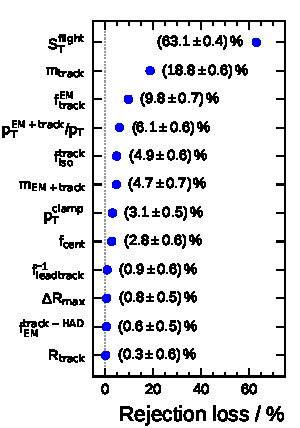
\includegraphics{./figures/bdt_perf/var_importance/3p_iter1.pdf}
    \subcaption{Iteration 1 (3-prong)}
  \end{subfigure}
  \caption{Variable importance. Averaged rejection loss over a gamma-tautau like
    dijet spectrum}
  \label{fig:variable_importance}
\end{figure}

One prong: Drop only ChPiEMEOverCaloEME \SI{0.7 +- 0.3}{\percent}

Three prong: Drop innerTrkAvgDist \SI{0.3 +- 0.6}{\percent}, then
ChPiEMEOverCaloEME \SI{1.2 +- 0.6}{\percent}, then etOverPtLeadTrk (do not drop)

Variable correlations, importance (dropped variables) \& dependence with
$p_\mathrm{T}$ (2D Hist - including pt), Variable Transformations (instead
of cutting out outliers), Partial Dependence, Including $p_\mathrm{T}$

\section{Identification Performance on Simulated Data}
\label{sec:bdt_perf}

\subsection{Performance in Simulation}
\label{sec:bdt_perf_sim}

\begin{figure}[ht]
  \begin{subfigure}[t]{0.48\textwidth}
    \centering
    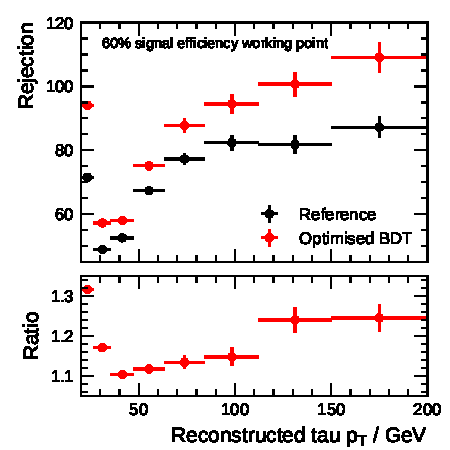
\includegraphics{./figures/bdt_perf/post_optimisation/rejection_1p.pdf}
    \subcaption{1-prong. (Dropped ChPiEMEOverCaloEME)}
  \end{subfigure}\hfill
  \begin{subfigure}[t]{0.48\textwidth}
    \centering
    \todo[inline]{3-prong Rejection}
    \subcaption{3-prong}
  \end{subfigure}
  \caption{Working points}
\end{figure}



\todo[inline]{Moneyplot: Rejection vs pt for tight working points after all
  improvements vs.\ old setup }

Impact on (reconstructed) decay modes (?)

\subsubsection{Performance on Quark- / Gluon-initiated Jets}
\label{sec:bdt_perf_quark_gluon}

Impact of Quark / Gluon initiated jets on Tau-ID (i.e. performance of ID
on Quark / Gluon jets)

\subsection{Performance on Data}
\label{sec:bdt_perf_data}

Performance on TAUP4 (?)

% -------------------------------------------------------------------------- %
\begin{itemize}
\item Description \& Plots of the input variables
  \begin{itemize}
  \item How does etOverPtLeadTrk differ from EMPOverTrkSysP for 1-prong taus?
  \end{itemize}

\item Train baseline for comparison (with default outlier removal)
  \begin{itemize}
  \item NTrees 100 (explain)
  \item MinNodeSize 0.1 (explain)
  \item BoostType AdaBoost (explain)
  \item SeparationType GiniIndex (explain)
  \item PruneMethod NoPruning
  \item UseYesNoLeaf False (explain)
  \item AdaBoostBeta 0.2 (explain)
  \item DoBoostMonitor True
  \item nCuts 200 (explain)
  \item MaxDepth 8 (explain)
  \end{itemize}

\item Variable transformations (log, clamp, uniformization)
  \begin{align}
    &\text{SumPtTrkFrac:} &\log(x + 10^{-4}) \\
    &\text{absipSigLeadTrk:} &\min(x, 30) \\
    &\text{mEflowApprox:} &\log(x) \\
    &\text{centFrac:} &\min(x, 1) \\
    &\text{innerTrkAvgDist:} &- \\
    &\text{ptRatioEflowApprox:} &\min(x, 4) \\
    &\text{EMPOverTrkSysP:} &\log(\max(10^{-3}, x)) \\
    &\text{etOverPtLeadTrk:} &\log(\max(0.1, x)) \\
    &\text{ChPiEMEOverCaloEME:} &\max(-4, \min(x, 5)) \\
    &\text{trFlightPathSig:} &\log(\max(0.01, x)) \\
    &\text{massTrkSys:} &\log(x) \\
    &\text{dRmax:} &-
  \end{align}

\item Variable importance (Google: Variable Importance Measures)
  \begin{itemize}
  \item Drop-one test
  \item Partial dependence (can we use a two way partial dependence plot to
    show interaction of pt and another variable?)
    \url{http://scikit-learn.org/stable/modules/ensemble.html#interpretation}
  \end{itemize}

\item $p_\mathrm{T}$-dependency 2D histograms of (centFrac / innerTrkAvgDist --
  worse \& SumPtTrkFrac -- should get better) (Plot 'variable separation' vs.
  pt)

\item Performance on gluon / quark initiated jets

\item Cross check with data (jets only)?

\end{itemize}

%%% Local Variables:
%%% mode: latex
%%% TeX-master: "mythesis"
%%% End:
